%! TEX root = course_report.tex

\section{Проектирование графического пользовательского интерфейса} % (fold)
\label{sec:gui_design}

Разработанное программное обеспечение представляет из себя библиотеку кода написанную на языках \fsharp{} и \csharp{}.
Библиотека предназначена для представления модификации классических байесовых сетей, упомянутой на странице~\pageref{page:domain:bayes_mod} в подразделе~\ref{sub:domain:bayes_net}.

\subsection{Обоснование проекта пользовательского интерфейса}
\label{sub:gui_design:motivation}

Так как в дипломном проекте рассматривается одна из разновидностей графовых моделей, то, очевидно, для представления таких моделей в разрабатываемой библиотеке должна быть часть, отвечающая за представление и работу с графами.
При реализации здесь было несколько альтернативных путей: использовать одну из доступных библиотек для платформы \dotnet{} для работы с графами или реализовать собственную.
Среди готовых библиотек можно было бы использовать QuickGraph\footnote{\url{http://quickgraph.codeplex.com/}}, Directed Graph for .NET\footnote{\url{http://directedgraph4net.codeplex.com/}} или GrapheNET\footnote{\url{http://graphenet.codeplex.com/}}.
Но было принято решение остановиться на варианте, подразумевающем разработку собственных типов для работы с графами.
Это решение было обосновано тем, что вышеуказанные библиотеки являются сложными и содержат в себе очень много функциональности не нужной для решения поставленных задач, в дополнение не было приобретено лишних мегабайтовых внешних зависимостей для библиотеки.

Одним из важных решений, которое было принято в начале проектирования модуля работы с графами, было использование по возможности неизменяемых структур данных.
Это решение выгодно отличает разработанную реализацию от существующих библиотек, от использования которых было принято решение отказаться. 
Существующие библиотеки ориентированы на работу в императивном стиле и с изменяемым состоянием.
Также использование неизменяемых структур данных для реализации типов для представления графов в дальнейшем положительно сказалось на простоте реализации поиска структуры вероятностной сети в алгоритмах вывода структуры по данным.
Часть разрабатываемой библиотеки, содержащая типы для работы с графами, реализована на языке программирования \fsharp{}.
Краткое описание основных особенностей данного языка приведено в подразделе~\ref{sub:practice:fsharp_overview}.
Решение использовать данный язык было продиктовано желанием сократить количество возможных ошибок и размер кодовой базы, необходимой для реализации поставленной задачи, а так же желанием применить в <<боевых>> условиях язык программирования с хорошей поддержкой функционального программирования.

Внутренним представлением графа является неизменяемый словарь, содержащий вложенный неизменяемый мульти"=словарь\footnote{Словарь позволяющий хранить множество значений с одинаковым ключом.}.
Основные определения структуры данных графа приведены в листинге~\ref{lst:arch_and_mod:graph_definition}:
\begin{lstlisting}[style=fsharpstyle,caption={Определение структуры данных для представления графа}, label=lst:arch_and_mod:graph_definition]
/// Graph arc 
type Arc<'T> =
    | Outgoing of 'T
    | Incoming of 'T

/// Immutable Graph class
[<ReferenceEquality; NoComparison>]
type Graph<'Vertex, 'Arc when 'Vertex : comparison and 'Vertex : equality and 'Vertex :> IComparable> = 
    private Graph of Map<'Vertex, MultiMap<'Vertex, Arc<'Arc>>>
\end{lstlisting}

Данная структура данных для представления графа подходит для работы как с неориентированными так и с ориентированными мультиграфами.
Воспринимать граф как ориентированный или нет задача конкретного алгоритма, работающего с графом.
Разработанная библиотека для представления графа предоставляет необходимые операции для манипулирования структурой графа. 
Библиотека также предоставляет небольшое количество алгоритмов для работы с графами, необходимых в рамках решения задач, возникающих при поиске структуры вероятностной сети.
В частности реализованы алгоритмы топологической сортировки, поиска в глубину и ширину, поиска сильно"=связанных компонетов и проверки графа на наличие направленных циклов. 

Одной из особенностей разработанной библиотеки является ориентированность на использование как из языка \fsharp{} в <<функциональном стиле>>, так и из языка \csharp{} "--- в <<императивном>>.
Для реализации данной возможности были учтены рекомендации приведенные в~\cite{fsdg_2010}.
Функциональность разработанной библиотеки покрыта большим набором модульных тестов, написанных с использованием библиотек xUnit\footnote{\url{http://xunit.codeplex.com/}} и Unquote\footnote{\url{http://code.google.com/p/unquote/}}.


\subsection{Представление вероятностной сети}
\label{sub:arch_and_mod:probab_net}

Другой важной частью разработанной библиотеки являются типы для представления и работы с самими вероятностными сетями.
Первостепенными требованиями, поставленными перед началом проектирования типов, были следующие пункты:
\begin{itemize}
  \item Типы предназначены для представления модификации классических байесовых сетей, упомянутой в разделе~\ref{sub:domain:bayes_net} на странице~\pageref{page:domain:bayes_mod}.
  \item Представление сети должно быть <<многослойным>>.
  Под <<многослойностью>> понимается возможность расширения представления сети дополнительными <<слоями>> атрибутов, с целью увеличения количества сценариев, в которых данные типы пригодны к использованию.
  Например, в случае когда нужно знать лишь структуру сети можно использовать лишь информацию о структуре "--- граф.
  Для проведения статистического вывода суждений добавляется дополнительный <<слой>>, содержащий талицы условных и безусловных вероятностей.
  В случаях, когда нужно отображать сеть пользователю, добавляется еще один <<слой>>, содержащий дополнительную информацию о переменных и их состояниях. 
  \item Сеть должна предоставлять возможность отмены вносимых в нее изменений, т.\,е. по сути поддерживать версионность.
  \item Сеть должна предоставлять возможность валидации её структуры. 
\end{itemize}

Приняв во внимание приведенные выше требования были приняты следующие решения:
\begin{itemize}
  \item Необходимо разработать отдельные типы для представления вершин вероятностной модели и связей между переменными в этой модели.
  В разработанной библиотеке за это отвечают типы \lstinline!Node<'T>! и \lstinline!Link<'T>!, содержащие информацию о переменных, таблицы распределения и дополнительные атрибуты.
  Использование параметрического полиморфизма в реализации данных типов играет ключевую роль в обеспечении <<многослойности>> и расширяемости представления вероятностной сети.
  \item Необходимы типы для представления распределения.
  В предложенной реализации был разработан тип для представления безусловного распределения случайной величины, эта таблица хранится в сети как один из аттрибутов типа \lstinline!Node<'T>!, и тип для представления условного распределения пары случайных величин, экземпляр данного типа хранится как аттрибут связи между переменными "--- \lstinline!Link<'T>!.
  Было сочтено целесообразным в качестве внутренней реализации таблиц распределения использовать готовую библиотеку для работы с матрицами и другими математическими объектами и понятиями "--- Math.NET Numerics\footnote{\url{http://numerics.mathdotnet.com/}}.
  Соответственно в предложенной реализации использовались типы \lstinline!Vector<float>! и \lstinline!Matrix<float>! и сопутствующие операции над ними.
  Использование данной библиотеки позволило сократить объём сопутствующего кода, необходимого для реализации библиотеки для работы с вероятностными сетями, также уменьшив множество потенциальных ошибок реализации.
  В данном случае преимущества от использования библиотеки превысили затраты на добавление и поддержку дополнительных зависимостей.

  \item Требование возможности отмены изменений вносимых в вероятностную сеть привело к реализации сети, как и в случае типов для представления графов, к реализации сети как неизменяемой структуры данных.
  Все операции, при условии использования специальных функций, возвращают новый экземпляр сети, оставляя старый не изменённым.
  Подобная реализация типов автоматически дает возможность производить версионирование экземпляров типа, т.\,к. всегда есть доступ к изменённой копии и исходному экземпляру.
  С первого взгляда данный подход кажется очень расточительным по памяти, но на самом деле оказывается, что все с точностью до наоборот, т.\,к. обычно, и в данном конкретном случае, при модификации неизменяемой структуры данных большая часть структуры разделяется между копией и исходной структурой, а физически копирование памяти происходит лишь в тех местах, которые действительно необходимо было поменять.
  Для убедительности, сказанное проиллюстрировано на рисунке~\ref{fig:arch_and_mod:probab_net:immutable_ds_modification}.

  \item Валидация сети происходит на этапе её построения и модификации.
  Дополнительно существуют функции для проверки структуры сети на ацикличность.
  Ацикличность ориентированного графа проверяется с помощью алгоритма нахождения компонент сильной связности Косарайю\footnote{\url{http://en.wikipedia.org/wiki/Kosaraju's_algorithm}}.

\end{itemize}

\begin{figure}[ht]
\centering
  \begin{subfigure}[b]{0.41\linewidth} 
    \centering
    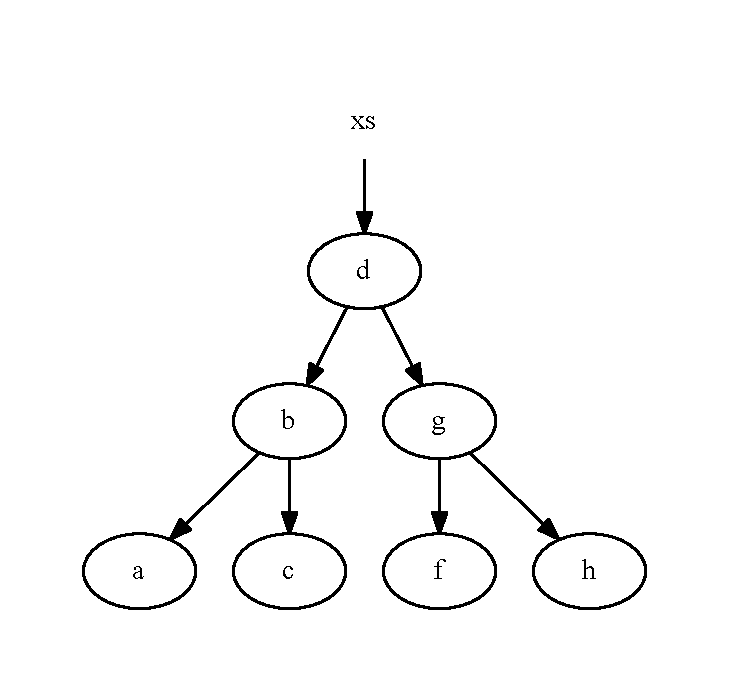
\includegraphics[scale=0.63]{persistent_tree.pdf}  
    \caption{}
  \end{subfigure}
  \begin{subfigure}[b]{0.58\linewidth} 
    \centering
    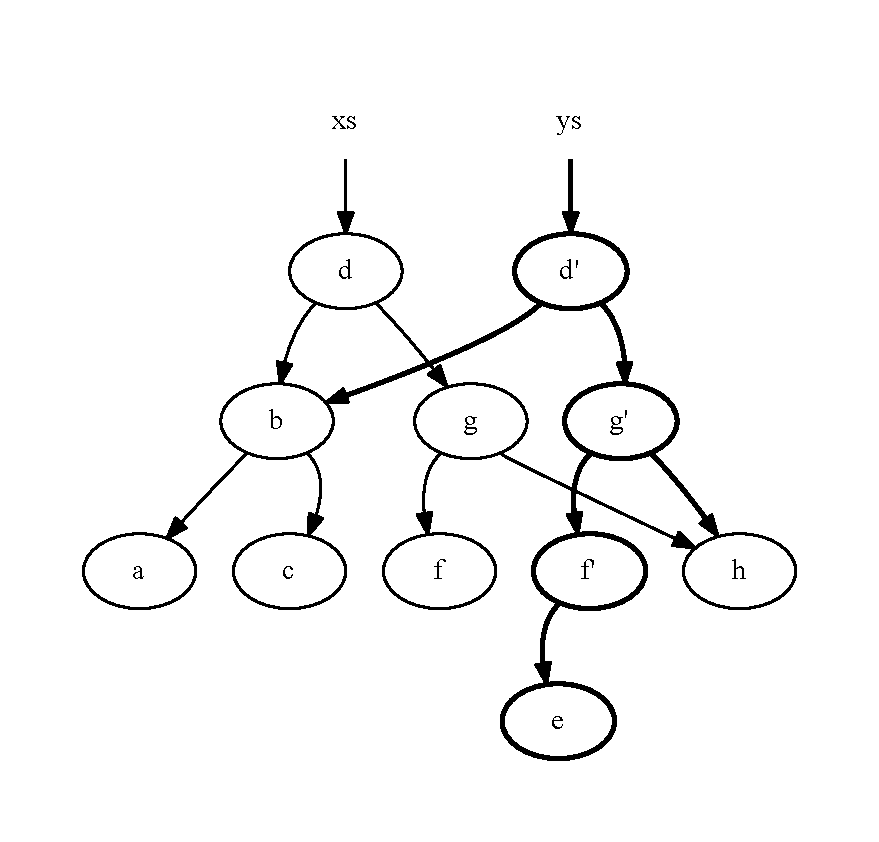
\includegraphics[scale=0.63]{persistent_tree_mod.pdf}  
    \caption{}
  \end{subfigure}
  \caption{ Пример разделения структуры в неизменяемых структурах данных: 
            а "--- исходное дерево;
            б "--- измененное дерево, добавлена вершина \textit{e};}
  \label{fig:arch_and_mod:probab_net:immutable_ds_modification}
\end{figure}

В результате получилось довольно простое и расширяемое представление сети, основное определение которого приведено в листинге~\ref{lst:arch_and_mod:probab_net:bnet_definition}.
Параметризация типа параметрами \lstinline!'NodeAttributes! и \lstinline!'LinkAttributes! и расширяемое устройство типов \lstinline!Node<'T>! и \lstinline!Link<'T>! позволяет достигнуть заявленной расширяемости представления сети и её <<многослойности>>.
Библиотека содержит предопредёленные типы, для представления уровней.
Параметризация типа \lstinline!BNet<unit, unit>! представляет структуру сети и таблицы распределения.
<<Слой>> с дополнительными аттрибутами, планируемыми для использования в алгоритмах статистического вывода суждений представлен типами \lstinline!NodeAttributes<'Annotations>! и \lstinline!LinkAttributes!, но на момент защиты дипломного проекта, из-за неготовой реализации алгоритмов статистического вывода суждений, данные типы содержат не все необходимые атрибуты для работы таких алгоритмов, а лишь прогнозируемых заготовки.
Дополнительный <<слой>>, потенциально необходимый при построении пользовательских приложений, представлен типом \lstinline!VarAnnotations!.
Данный тип содержит дополнительную информацию о переменной, такую как её название и аннотации возможных значений переменной.
Таким образом, наиболее полное представление сети, содержащее все <<слои>>, в коде параметризуется следующим образом \lstinline!BNet<NodeAttributes<VarAnnotations>, LinkAttributes>!.

\begin{lstlisting}[style=fsharpstyle,caption={Определение структуры данных для вероятностной сети}, label=lst:arch_and_mod:probab_net:bnet_definition]
/// Represents immutable BN. Nodes and links between nodes.
type BNet<'NodeAttributes, 'LinkAttributes> = 
    private { nodes: Map<int, Node<'NodeAttributes>>;
              links: Map<int * int, Link<'LinkAttributes>>;
              graph: Graph<int, unit>; } 
\end{lstlisting}

Таким образом, использование параметрического полиморфизма и не\-изменяемых типов данных, позволило добиться поставленных при проектировании целей, а также довольно легкой возможности расширять сеть в дальнейшем.

\subsection{Сохранение сети} % (fold)
\label{sub:arch_and_mod:net_persistence}

Помимо функциональности, связанной с представлением, манипуляцией и выведением структуры сети, разработанная библиотека предоставляет возможность импорта и экспорта вероятностной сети из и в различные форматы.
Т.\,к. библиотека предназначена для работы с модификацией вероятностных сетей, отличающейся в нескольких ключевых моментах от классических байесовых сетей, то нельзя было использовать общепринятые форматы для хранения сетей во внешней памяти и необходимо было разработать свой формат.
Разработанный формат хранения сетей основывается на XML и предназначен для полного сохранения состояния представления сети, используемого в программе.
Данный формат в большей степени похож на ручную сериализацию, чем на удобный формат для обмена вероятностными сетями.
Пример сети, представленной в данном формате, приведен в листинге~\ref{lst:arch_and_mod:net_persistence:bnxml}.

У разработанного формата есть существенный недостаток, его <<понимает>> только разработанная библиотека.
В связи с тем, что в данном дипломном проекте основной целью является реализация лишь малой части возможных операций над вероятностными сетями "--- построение структуры по данным, целесообразно было добавить в библиотеку, хотя и весьма ограниченную, возможность загрузки и сохранения вероятностных сетей из и в существующие распространённые форматы.
Список поддерживаемых форматов приведён в таблице~\ref{table:arch_and_mod:net_persistence:supported_formats}.
Поддержка нескольких форматов понадобилась потому, что многие существующие программы, которые использовались в различной степени для оценки результатов проделанной работы, поддерживают весьма ограниченный набор форматов.
Таким образом, имея возможность экспортировать сеть, построенную одним из алгоритмов реализованных в разработанной библиотеке по данным, в общеиспользуемый формат можно использовать обученную сеть для статистического вывода суждений и других операций в существующих программах, т.\,к. в данный момент в разработанной библиотеке данная функциональность не реализована.
Отдельно стоит отметить возможность сохранения структуры сети в формат представления графов программы GraphViz\footnote{\url{http://www.graphviz.org/}}.
Данное ПО использовалось с целью визуализации выведенных структур и экспорта полученной визуализации в один из векторных графических форматов.
Утилита dot из состава GraphViz умеет автоматически визуализировать сложные графы наилучшим для отображения образом.

\clearpage
\begin{lstlisting}[language=XML,caption={Пример представления простой вероятностной сети в собственном XML"=формате}, label=lst:arch_and_mod:net_persistence:bnxml]
<network>
  <variables>
    <variable id="1" dim="2" />
    <variable id="2" dim="3" />
  </variables>
  <node_attributes>
    <node variable_id="1"> <answered>false</answered> </node>
    <node variable_id="2"> <answered>true</answered>  </node>
  </node_attributes> 
  <link_attributes>
    <link parent_id="1" child_id="2" />
  </link_attributes>
  <variable_annotations>
    <variable_annotation variable_id="1">
      <name>My variable</name>
      <annotations>
        <label>Yes</label> <label>No</label>
      </annotations>
    </variable_annotation>
    <variable_annotation variable_id="2">
      <name>Color</name>
      <annotations>
        <label>Red</label> <label>Green</label> <label>Blue</label>
      </annotations>
    </variable_annotation>
  </variable_annotations>
  <probability_tables>
    <probability_table variable_id="1">
      <vector>0.2 0.8</vector>
    </probability_table>
    <probability_table variable_id="2">
      <vector>0.4 0.3 0.3</vector>
    </probability_table>
  </probability_tables>
  <forward_probability_tables>
    <forward_probability_table variable_id="2" condition_variable_id="1">
      <matrix nrows="3" ncols="2">0.1 0.2 0.7 0.6 0.1 0.3</matrix>
    </forward_probability_table>
  </forward_probability_tables>
</network>
\end{lstlisting}

\begin{table}[ht]
\caption{Поддерживаемые форматы хранения вероятностных сетей}
\label{table:arch_and_mod:net_persistence:supported_formats}
\centering
  \begin{tabular}{| >{\raggedright}m{0.35\textwidth} 
                  | >{\centering}m{0.27\textwidth} 
                  | >{\centering\arraybackslash}m{0.27\textwidth}|}
  \hline Формат & Поддержка импорта & Поддержка экспорта \\
  \hline Собственный xml"=формат & полная & полная \\
  \hline XMLBIF & частичная & частичная \\
  \hline GeNIe & частичная & отсутствует \\
  \hline GraphViz dot & отсутствует & полная \\
  \hline
  \end{tabular}
\end{table}
